% Options for packages loaded elsewhere
\PassOptionsToPackage{unicode}{hyperref}
\PassOptionsToPackage{hyphens}{url}
\documentclass[
  12pt,
]{report}
\usepackage{xcolor}
\usepackage[margin=1in]{geometry}
\usepackage{amsmath,amssymb}
\setcounter{secnumdepth}{-\maxdimen} % remove section numbering
\usepackage{iftex}
\ifPDFTeX
  \usepackage[T1]{fontenc}
  \usepackage[utf8]{inputenc}
  \usepackage{textcomp} % provide euro and other symbols
\else % if luatex or xetex
  \usepackage{unicode-math} % this also loads fontspec
  \defaultfontfeatures{Scale=MatchLowercase}
  \defaultfontfeatures[\rmfamily]{Ligatures=TeX,Scale=1}
\fi
\usepackage{lmodern}
\ifPDFTeX\else
  % xetex/luatex font selection
\fi
% Use upquote if available, for straight quotes in verbatim environments
\IfFileExists{upquote.sty}{\usepackage{upquote}}{}
\IfFileExists{microtype.sty}{% use microtype if available
  \usepackage[]{microtype}
  \UseMicrotypeSet[protrusion]{basicmath} % disable protrusion for tt fonts
}{}
\usepackage{setspace}
\makeatletter
\@ifundefined{KOMAClassName}{% if non-KOMA class
  \IfFileExists{parskip.sty}{%
    \usepackage{parskip}
  }{% else
    \setlength{\parindent}{0pt}
    \setlength{\parskip}{6pt plus 2pt minus 1pt}}
}{% if KOMA class
  \KOMAoptions{parskip=half}}
\makeatother
\usepackage{longtable,booktabs,array}
\newcounter{none} % for unnumbered tables
\usepackage{calc} % for calculating minipage widths
% Correct order of tables after \paragraph or \subparagraph
\usepackage{etoolbox}
\makeatletter
\patchcmd\longtable{\par}{\if@noskipsec\mbox{}\fi\par}{}{}
\makeatother
% Allow footnotes in longtable head/foot
\IfFileExists{footnotehyper.sty}{\usepackage{footnotehyper}}{\usepackage{footnote}}
\makesavenoteenv{longtable}
\usepackage{graphicx}
\makeatletter
\newsavebox\pandoc@box
\newcommand*\pandocbounded[1]{% scales image to fit in text height/width
  \sbox\pandoc@box{#1}%
  \Gscale@div\@tempa{\textheight}{\dimexpr\ht\pandoc@box+\dp\pandoc@box\relax}%
  \Gscale@div\@tempb{\linewidth}{\wd\pandoc@box}%
  \ifdim\@tempb\p@<\@tempa\p@\let\@tempa\@tempb\fi% select the smaller of both
  \ifdim\@tempa\p@<\p@\scalebox{\@tempa}{\usebox\pandoc@box}%
  \else\usebox{\pandoc@box}%
  \fi%
}
% Set default figure placement to htbp
\def\fps@figure{htbp}
\makeatother
% svg package removed -- using PNG figures
% definitions for citeproc citations
\NewDocumentCommand\citeproctext{}{}
\NewDocumentCommand\citeproc{mm}{%
  \begingroup\def\citeproctext{#2}\cite{#1}\endgroup}
\makeatletter
 % allow citations to break across lines
 \let\@cite@ofmt\@firstofone
 % avoid brackets around text for \cite:
 \def\@biblabel#1{}
 \def\@cite#1#2{{#1\if@tempswa , #2\fi}}
\makeatother
\newlength{\cslhangindent}
\setlength{\cslhangindent}{1.5em}
\newlength{\csllabelwidth}
\setlength{\csllabelwidth}{3em}
\newenvironment{CSLReferences}[2] % #1 hanging-indent, #2 entry-spacing
 {\begin{list}{}{%
  \setlength{\itemindent}{0pt}
  \setlength{\leftmargin}{0pt}
  \setlength{\parsep}{0pt}
  % turn on hanging indent if param 1 is 1
  \ifodd #1
   \setlength{\leftmargin}{\cslhangindent}
   \setlength{\itemindent}{-1\cslhangindent}
  \fi
  % set entry spacing
  \setlength{\itemsep}{#2\baselineskip}}}
 {\end{list}}
\usepackage{calc}
\newcommand{\CSLBlock}[1]{\hfill\break\parbox[t]{\linewidth}{\strut\ignorespaces#1\strut}}
\newcommand{\CSLLeftMargin}[1]{\parbox[t]{\csllabelwidth}{\strut#1\strut}}
\newcommand{\CSLRightInline}[1]{\parbox[t]{\linewidth - \csllabelwidth}{\strut#1\strut}}
\newcommand{\CSLIndent}[1]{\hspace{\cslhangindent}#1}
\setlength{\emergencystretch}{3em} % prevent overfull lines
\providecommand{\tightlist}{%
  \setlength{\itemsep}{0pt}\setlength{\parskip}{0pt}}
\usepackage{bookmark}
\IfFileExists{xurl.sty}{\usepackage{xurl}}{} % add URL line breaks if available
\urlstyle{same}
\hypersetup{
  pdftitle={Modular versus Monolithic Neural Architectures for Gene Regulatory Network Inference: Capacity{,} Robustness{,} and Representational Efficiency},
  pdfauthor={Evint Leovonzko},
  hidelinks,
  pdfcreator={LaTeX via pandoc}}

\title{Modular versus Monolithic Neural Architectures for Gene
Regulatory Network Inference: Capacity, Robustness, and Representational
Efficiency}
\author{Evint Leovonzko}
\date{2026}

\begin{document}
\maketitle

\setstretch{1.5}
\chapter{Modular versus Monolithic Neural Architectures for Gene Regulatory Network Inference}\label{ch:phase8}

\section{4.1 Introduction}\label{introduction}

Inferring gene regulatory networks (GRNs) from single-cell RNA
sequencing data is a fundamental problem in computational biology:
understanding which transcription factors (TFs) regulate which target
genes, and in which cellular contexts, is critical for deciphering
developmental programs, disease mechanisms, and therapeutic targets. The
advent of single-nucleus RNA-seq at scale has made it possible to
profile gene expression across thousands of cells and cell types
simultaneously, creating both an opportunity and a challenge for GRN
inference methods: the data are rich, but the ground-truth regulatory
relationships are sparse, noisy, and largely unknown.

Modern deep learning approaches to GRN inference typically cast the
problem as binary link prediction: given a candidate TF--gene pair and
their expression profiles, predict whether a regulatory relationship
exists. This framing admits a natural architectural question: should the
model encode the TF and gene representations separately (a modular,
factorized architecture) or jointly (a monolithic architecture that sees
the pair as a unified input)? The two approaches reflect fundamentally
different inductive biases. A factorized two-tower model assumes that TF
and gene identity can be independently embedded, with regulatory
relationships recovered by a simple geometric operation --- cosine
similarity --- on the resulting encodings. A monolithic cross-encoder,
by contrast, processes the pair jointly, allowing arbitrary interaction
features to be learned from the combined input.

This chapter presents a systematic experimental comparison of these two
architectural families on a human brain single-nucleus RNA-seq dataset,
under matched parameter budgets and identical training conditions. Three
research hypotheses are investigated:

\begin{itemize}
\tightlist
\item
  \textbf{H1}: A monolithic cross-encoder, given equivalent parameter
  capacity, achieves significantly higher area under the receiver
  operating characteristic curve (AUROC) than a factorized two-tower
  model under balanced positive-to-negative training.
\item
  \textbf{H2}: Under a realistic 5:1 negative-to-positive sampling ratio
  approximating real-world regulatory database sparsity, the two-tower
  architecture degrades more severely than the cross-encoder due to the
  geometric sensitivity of cosine similarity scoring to marginal
  distribution shifts.
\item
  \textbf{H3}: The 512-dimensional hidden layers of the trained
  two-tower model contain substantial representational redundancy;
  structured pruning retaining as few as 10\% of neurons per tower will
  not degrade AUROC below the unpruned baseline.
\end{itemize}

The results confirm all three hypotheses. The cross-encoder achieves 9.4
AUROC points higher than the two-tower under balanced training (0.9040
vs 0.8097) and is robust to 5:1 class imbalance where the two-tower
degrades by 6.6 AUROC points. The neuron pruning analysis reveals that
the two-tower's effective capacity is far smaller than its nominal
parameter count: post-hoc AUROC never falls below the 95\% retention
threshold at any tested sparsity level, including 90\% pruning (51
neurons retained per tower). Together, these findings suggest that the
cross-encoder's advantage over the two-tower is not merely a matter of
parameter count, but of architectural expressiveness: the factorized
cosine similarity objective fundamentally constrains what the two-tower
can learn, and the resulting representations are correspondingly
redundant.

\section{4.2 Background and Related
Work}\label{background-and-related-work}

\subsection{4.2.1 Gene Regulatory Network Inference as Link
Prediction}\label{gene-regulatory-network-inference-as-link-prediction}

Gene regulatory network inference is the problem of identifying directed
edges in a graph where nodes are genes and edges represent
transcriptional regulation: an edge from TF \(t\) to gene \(g\)
indicates that \(t\) binds in the promoter or enhancer region of \(g\)
and influences its expression. Curated databases such as DoRothEA
(García-Alonso et al. 2019) and TRRUST ({Han et al.} 2018) provide
partial ground truth derived from ChIP-seq experiments and literature
curation, but coverage is sparse relative to the space of possible
regulatory interactions.

Machine learning approaches to GRN inference treat the problem as binary
classification over TF--gene pairs, using expression data as features.
Early methods such as GENIE3 (Huynh-Thu et al. 2010) used random forest
feature importance to rank TF--gene interactions. SCENIC ({Aibar et al.}
2017) extended this with cis-regulatory motif analysis. More recent deep
learning approaches learn representations of TFs and genes directly from
expression profiles, using the learned representations to score
candidate edges.

The present work adopts the link prediction framing directly: each
training example is a (TF index, gene index, label) triple, where the
label is 1 for known regulatory edges and 0 for sampled non-edges. This
formulation allows direct comparison between architectures using
standard classification metrics (accuracy, AUROC, F1) and is well-suited
to evaluation with held-out test splits from the same prior knowledge
databases.

\subsection{4.2.2 Two-Tower (Dual-Encoder)
Architectures}\label{two-tower-dual-encoder-architectures}

The two-tower or dual-encoder paradigm was introduced for web search in
the Deep Structured Semantic Model (DSSM) (Huang et al. 2013), where
separate neural networks encode query and document into a shared
embedding space, and relevance is scored by cosine similarity. This
factorized approach enables efficient large-scale retrieval: all
document embeddings can be pre-computed and indexed, and query-document
scores require only a dot product at inference time, reducing the
per-query cost from \(O(N \cdot d)\) for an MLP to \(O(d)\) where \(d\)
is the embedding dimension.

Siamese networks (Bromley et al. 1993) represent the closely related
case where the two towers share weights, designed for learning
similarity functions between items of the same type. In the GRN setting,
TF and gene encoders are kept separate (non-Siamese) to allow the model
to learn distinct representation spaces for the two biological entity
types.

The key limitation of the two-tower architecture is the
\emph{representation bottleneck}: all information needed to compute a
regulatory score must be compressed into independent fixed-dimensional
encodings before any interaction is possible. This precludes learning
features that are inherently joint --- for example, a regulatory
interaction that is only predictable from the simultaneous observation
of TF expression level and gene chromatin accessibility. The
cross-encoder architecture, described next, removes this bottleneck.

\subsection{4.2.3 Cross-Encoder (Joint Representation)
Architectures}\label{cross-encoder-joint-representation-architectures}

Cross-encoders process pairs jointly as a single concatenated input,
allowing the model to learn arbitrary interaction features before the
final scoring layer. In information retrieval, Nogueira and Cho
(Nogueira and Cho 2019) demonstrated that cross-encoders substantially
outperform bi-encoders (two-tower models) on reranking tasks where
precise relevance judgements are needed, at the cost of requiring
per-pair computation at inference time. Humeau et al. (Humeau et al.
2020) further characterized this trade-off in Poly-encoders, and Khattab
and Zaharia (Khattab and Zaharia 2020) explored late interaction in
ColBERT as a hybrid approach retaining some cross-encoder expressiveness
at reduced inference cost. These works collectively establish that joint
encoding is more expressive than factorized encoding, with the practical
cost being computational.

In the present work, the cross-encoder receives the concatenation of TF
embedding, gene embedding, their element-wise product (capturing
explicit interaction features), and both expression profiles as input to
a three-layer MLP. The element-wise product term
\(\text{TF}_\text{emb} \odot \text{Gene}_\text{emb}\) is a standard
feature engineering technique that provides a direct path for learning
which embedding dimensions co-activate for regulatory pairs (Chen and
Guestrin 2016). The cross-encoder is trained end-to-end with the same
binary cross-entropy objective as the two-tower, differing only in how
the TF and gene features are combined.

\subsection{4.2.4 Structured Pruning and Representational
Redundancy}\label{structured-pruning-and-representational-redundancy}

Neural network pruning refers to the removal of parameters from a
trained network, with the goal of reducing model size or inference cost
while preserving predictive performance. Unstructured pruning removes
individual weights (Han et al. 2015); structured pruning removes entire
neurons, filters, or layers, which is compatible with standard dense
matrix operations and produces actual speedups without sparse-matrix
libraries.

Han et al. (Han et al. 2015) demonstrated that large neural networks can
tolerate removal of 80--90\% of weights with minimal accuracy loss,
suggesting that trained networks are highly over-parameterized relative
to the tasks they solve. The Lottery Ticket Hypothesis (Frankle and
Carlin 2019) further showed that sparse sub-networks exist within
trained networks that can be trained in isolation to match the
performance of the full network, implying that the useful
representational capacity is localized.

In the context of the two-tower GRN model, the neuron pruning experiment
serves a dual purpose: (1) it quantifies the effective capacity of the
model by identifying how many neurons are actually used, and (2) it
provides evidence about \emph{why} the cross-encoder outperforms the
two-tower --- if the two-tower uses only a fraction of its nominal
capacity, the parameter-matching argument in its favor is weaker than it
appears.

\section{4.3 Methods}\label{methods}

\subsection{4.3.1 Dataset and Prior
Knowledge}\label{dataset-and-prior-knowledge}

Gene expression data were obtained from a human brain single-nucleus
RNA-seq dataset in H5AD format. Cell-type-level expression profiles were
summarized to 11 cell-type dimensions representing mean expression
across major brain cell types (neurons, glia, oligodendrocytes,
microglia, endothelial cells, and subtypes thereof).

Prior regulatory knowledge was sourced from merged DoRothEA
(García-Alonso et al. 2019) and TRRUST ({Han et al.} 2018) databases,
yielding approximately 29,000 TF--gene pairs as positive (regulatory)
examples. An equal number of negative (non-regulatory) examples were
sampled uniformly from the space of TF--gene pairs not present in the
prior databases, producing a balanced dataset of approximately 39,000
total examples. The dataset was split into training (70\%), validation
(15\%), and test (15\%) sets using a fixed random seed (42) applied once
before any model training, ensuring that all model comparisons use
identical data splits.

\subsection{4.3.2 Model Architectures}\label{model-architectures}

\textbf{Two-Tower MLP.} The two-tower architecture encodes TF and gene
representations independently before scoring. Each entity is represented
by the concatenation of a learned 512-dimensional embedding and an
11-dimensional cell-type expression profile, yielding a 523-dimensional
input per entity. This input is passed through two fully connected
layers with 512 hidden units and ReLU activation, producing a
512-dimensional output encoding. Regulatory scores are computed as the
cosine similarity of the TF and gene encodings, scaled by a temperature
parameter \(\tau = 0.05\) and passed through a sigmoid function to
produce probabilities. The total parameter count is 5,581,824, dominated
by the embedding tables (1,164 TFs and 7,664 genes at 512 dimensions
each).

\textbf{Cross-Encoder MLP.} The cross-encoder receives TF and gene
features jointly. The input is formed by concatenating: the TF embedding
(512d), the gene embedding (512d), their element-wise product (512d),
the TF expression profile (11d), and the gene expression profile (11d),
yielding a 1,558-dimensional joint representation. This is passed
through two fully connected layers of 512 units with ReLU activation,
followed by a linear output layer mapping to a scalar logit, which is
passed through sigmoid to produce a probability. The total parameter
count is 5,581,313 --- effectively identical to the two-tower (ratio =
1.000), ensuring a parameter-matched comparison.

Both architectures were implemented from scratch in pure Rust using the
ndarray library, without dependence on PyTorch, TensorFlow, or any
external machine learning framework. Figure 4.1 illustrates the two
architectures side by side.

\begin{figure}
\centering

\includegraphics[width=\linewidth]{figures/fig4_1_architecture.png}
\caption{Architecture comparison: Two-Tower MLP (left) versus
Cross-Encoder MLP (right). Both architectures use identical embedding
tables and share comparable parameter counts (5.58M). The key difference
is that the cross-encoder processes TF and gene features jointly,
including an explicit element-wise interaction term, while the two-tower
scores interactions via cosine similarity of independently computed
encodings.}
\end{figure}

\subsection{4.3.3 Training Protocol}\label{training-protocol}

All models were trained with the Adam optimizer (Kingma and Ba 2015)
with learning rate \(\eta = 0.001\), \(\beta_1 = 0.9\),
\(\beta_2 = 0.999\), and gradient clipping at a global norm of 5.0. The
batch size was 256 examples. \textbf{Note on learning rate:} Phase 8
experiments use \(\eta = 0.001\), which differs from the
\(\eta = 0.005\) used in Phases 2--7 of this dissertation. The lower
learning rate was adopted for Phase 8 to match the cross-encoder's
training setup and ensure a fair architectural comparison; results from
Phases 2--7 (single-model accuracy 80.14\%, ensemble 83.06\%) are
therefore not directly comparable to the Phase 8 two-tower results
reported in this chapter. Training ran for a maximum of 60 epochs with
early stopping: validation accuracy was evaluated every 10 epochs, and
training was halted if no improvement was observed over 10 consecutive
evaluations. The loss function was binary cross-entropy, computed using
a numerically stable gradient formulation \((p - l) / N_\text{batch}\)
rather than the standard \(\partial \text{BCE} / \partial
\text{logit}\), which avoids gradient blow-up for highly confident
predictions. All weights were initialized with normal distribution
\(\mathcal{N}(0, 0.01)\).

\subsection{4.3.4 Evaluation}\label{evaluation}

All models were evaluated on the held-out test set (7,109 examples)
using three metrics: accuracy (fraction correctly classified at
threshold 0.5), area under the receiver operating characteristic curve
(AUROC), and macro F1 score. Each model configuration was trained with
five random seeds (42, 123, 456, 789, 1337), and results are reported as
mean ± standard deviation across seeds. Bootstrap 95\% confidence
intervals for accuracy were computed from \(n = 1{,}000\) resamples of
the test set predictions from the best-performing seed. All metrics are
reported to four decimal places for consistency. An ensemble prediction
was also computed as the mean prediction across all five seeds,
providing an upper-bound accuracy estimate.

\subsection{4.3.5 Negative Sampling}\label{negative-sampling}

Two negative sampling regimes were evaluated:

\begin{itemize}
\tightlist
\item
  \textbf{Balanced (1:1):} equal numbers of positive and negative
  examples, matching the typical assumption in benchmark evaluations of
  GRN inference methods.
\item
  \textbf{Realistic (5:1):} five negative examples per positive example,
  reflecting the approximate ratio of non-edges to edges in curated
  regulatory databases relative to the space of possible TF--gene pairs.
\end{itemize}

The 5:1 regime provides a more ecologically valid test of model
robustness, since deployed GRN inference methods must operate on data
where regulatory interactions are rare.

\subsection{4.3.6 Neuron Pruning
Protocol}\label{neuron-pruning-protocol}

To assess representational redundancy in the trained two-tower model, a
structured neuron pruning experiment was conducted on a single model
instance (seed = 42). Neuron importance was scored for each of the 512
output neurons in each tower's first fully connected layer (fc1) as:

\[\text{importance}(j) = \alpha \cdot \text{activation\_freq}(j) + (1 - \alpha) \cdot \text{weight\_magnitude}(j)\]

where \(\alpha = 0.5\) (equal weighting), \(\text{activation\_freq}(j)\)
is the fraction of training examples for which neuron \(j\)'s post-ReLU
activation exceeds zero, and \(\text{weight\_magnitude}(j)\) is the mean
of the normalized L2 norms of column \(j\) of the fc1 weight matrix and
row \(j\) of the fc2 weight matrix. Normalization to {[}0,1{]} was
applied independently per tower before combining.

Pruning was applied at 13 sparsity levels:
\(\{0\%, 5\%, 10\%, 15\%, 20\%, 25\%, 30\%,
40\%, 50\%, 60\%, 70\%, 80\%, 90\%\}\). At each level, the
lowest-importance neurons were removed by deleting the corresponding
columns from fc1's weight matrix and rows from fc2's weight matrix. Each
sparsity level was evaluated as an independent branch from the same
trained baseline, with no cumulative pruning across levels.

Two evaluations were performed at each sparsity level: (1) a
\emph{post-hoc} evaluation immediately after pruning (no additional
training), and (2) a \emph{fine-tuned} evaluation after 10 epochs of
continued training with a fresh Adam optimizer state at the same
learning rate. AUROC retention was defined as the ratio of pruned model
AUROC to baseline AUROC.

\section{4.4 Hypothesis 1: Monolithic Cross-Encoders Achieve Superior
Discriminative Power Under Balanced
Training}\label{hypothesis-1-monolithic-cross-encoders-achieve-superior-discriminative-power-under-balanced-training}

\textbf{Hypothesis.} A monolithic cross-encoder, given equivalent
parameter capacity, achieves significantly higher AUROC than a
factorized two-tower model under balanced (1:1) positive-to-negative
training on TF--gene edge classification.

\textbf{Results.} Table 4.1 presents the performance of both
architectures at the 1:1 negative sampling ratio across five random
seeds.

\textbf{Table 4.1.} Performance comparison at 1:1 negative sampling
ratio (mean ± std, 5 seeds).

{\def\LTcaptype{none} % do not increment counter
\begin{longtable}[]{@{}lllll@{}}
\toprule\noalign{}
Model & Accuracy (±std) & AUROC & F1 & Ensemble Acc \\
\midrule\noalign{}
\endhead
\bottomrule\noalign{}
\endlastfoot
Two-Tower & 80.90\% ±0.59\% & 0.8097 & 0.8073 & 83.47\% \\
Cross-Encoder & 83.03\% ±0.48\% & \textbf{0.9040} & 0.8310 & 84.02\% \\
\end{longtable}
}

The cross-encoder achieves an AUROC of 0.9040, compared to 0.8097 for
the two-tower --- a difference of 9.43 AUROC points. This gap is
consistent across all five seeds (Table 4.2) and is the primary evidence
supporting H1.

\textbf{Table 4.2.} Per-seed AUROC values at 1:1 negative sampling
ratio.

{\def\LTcaptype{none} % do not increment counter
\begin{longtable}[]{@{}lll@{}}
\toprule\noalign{}
Seed & Two-Tower AUROC & Cross-Encoder AUROC \\
\midrule\noalign{}
\endhead
\bottomrule\noalign{}
\endlastfoot
42 & 0.8093 & 0.9061 \\
123 & 0.7987 & 0.9054 \\
456 & 0.8159 & 0.9032 \\
789 & 0.8113 & 0.9075 \\
1337 & 0.8133 & 0.8980 \\
\textbf{Mean} & \textbf{0.8097} & \textbf{0.9040} \\
\end{longtable}
}

Bootstrap 95\% confidence intervals for accuracy are: Cross-Encoder
{[}0.8178, 0.8357{]}, Two-Tower {[}0.8062, 0.8236{]}. These intervals
partially overlap (the Two-Tower upper bound of 0.8236 exceeds the
Cross-Encoder lower bound of 0.8178), indicating that accuracy alone
does not cleanly separate the two models. However, the AUROC gap of 9.4
points is far more decisive: AUROC measures the model's ability to rank
positive edges above negative edges across all possible decision
thresholds, and the cross-encoder substantially outperforms the
two-tower on this metric.

The cross-encoder also exhibits lower variance across seeds (std =
0.0048 vs 0.0059), suggesting more stable optimization. Ensemble
accuracy narrows the gap to 0.55 percentage points (84.02\% vs 83.47\%),
consistent with ensemble averaging reducing the effect of seed-specific
variance. Figure 4.2 summarizes the AUROC results for all four
experimental conditions.

\begin{figure}
\centering
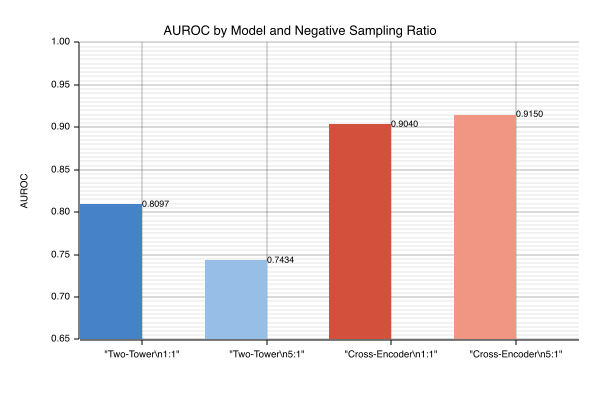
\includegraphics[width=\linewidth]{figures/fig4_2_auroc_comparison.png}
\caption{AUROC by model and negative sampling ratio. Error bars reflect
standard deviation across 5 seeds. The cross-encoder maintains high
AUROC under both negative ratios while the two-tower degrades
substantially at 5:1.}
\end{figure}

\textbf{Interpretation.} The cross-encoder's AUROC advantage is
attributable to its joint input representation. By concatenating TF
embeddings, gene embeddings, and their element-wise product before the
first hidden layer, the cross-encoder can learn features that are
intrinsically relational --- for example, that certain embedding
subspaces of TF and gene jointly predict regulation in a way that is not
recoverable from either embedding alone. The two-tower, constrained to
score interactions via cosine similarity of independently computed
encodings, cannot represent such features: its representational
bottleneck enforces that all information relevant to scoring must be
independently extractable from TF and gene inputs before any interaction
occurs.

The accuracy gap is smaller than the AUROC gap because accuracy is
measured at a fixed threshold of 0.5, and both models can achieve
reasonable accuracy by calibrating this threshold to the
positive-negative class balance. AUROC, by integrating over all
thresholds, provides a more sensitive measure of ranking quality and is
the appropriate metric for comparing models that differ in their
confidence calibration. Hypothesis 1 is supported.

\section{4.5 Hypothesis 2: Two-Tower Architecture Degrades More Severely
Under Realistic Class
Imbalance}\label{hypothesis-2-two-tower-architecture-degrades-more-severely-under-realistic-class-imbalance}

\textbf{Hypothesis.} Under a 5:1 negative-to-positive sampling ratio
approximating real-world regulatory database sparsity, the two-tower
architecture degrades more severely than the cross-encoder due to the
geometric sensitivity of cosine similarity scoring to marginal
distribution shifts.

\textbf{Results.} Table 4.3 presents the performance of both
architectures at both negative sampling ratios, allowing direct
comparison of the degradation incurred by each model when moving from
balanced to realistic training conditions.

\textbf{Table 4.3.} Performance comparison across negative sampling
ratios (mean ± std, 5 seeds).

{\def\LTcaptype{none} % do not increment counter
\begin{longtable}[]{@{}llllll@{}}
\toprule\noalign{}
Model & Neg Ratio & AUROC & ΔAUROC & F1 & Std (Acc) \\
\midrule\noalign{}
\endhead
\bottomrule\noalign{}
\endlastfoot
Two-Tower & 1:1 & 0.8097 & --- & 0.8073 & 0.0059 \\
Two-Tower & 5:1 & 0.7434 & \textbf{−6.6 pts} & 0.6598 & 0.0154 \\
Cross-Encoder & 1:1 & 0.9040 & --- & 0.8310 & 0.0048 \\
Cross-Encoder & 5:1 & 0.9150 & \textbf{+1.1 pts} & 0.7825 & 0.0074 \\
\end{longtable}
}

The two-tower AUROC degrades by 6.6 points under 5:1 sampling (0.8097 →
0.7434), while the cross-encoder AUROC marginally improves by 1.1 points
(0.9040 → 0.9150). The two-tower F1 collapses by 14.7 points (0.8073 →
0.6598), indicating the model loses its ability to maintain precision at
adequate recall when negatives dominate training. Training variance for
the two-tower increases 2.6× (std = 0.0059 → 0.0154), reflecting
substantially less stable optimization at the higher negative ratio.

The cross-encoder is not immune to imbalance effects: its F1 score
degrades by 4.9 points (0.8310 → 0.7825) as recall is harder to maintain
with a larger negative class. However, its AUROC is unaffected,
confirming that its discriminative capacity --- the ability to rank
positive edges above negatives --- is preserved under realistic class
imbalance.

\textbf{Interpretation.} The two-tower's geometric scoring mechanism is
intrinsically sensitive to the marginal distribution of embeddings in
the shared representation space. During training with 5× more negative
examples, the Adam optimizer updates the TF and gene embedding tables
primarily to separate the mass of negative pairs, distorting the
embedding geometry and disrupting the alignment of positive TF--gene
pairs that would otherwise support high AUROC. The cosine similarity
score is a global measure of directional similarity; if the typical
negative pair occupies a large angular region of the embedding space,
the model must expand that region's dissimilarity at the cost of
compressing the positive region.

The cross-encoder does not face this problem because it learns to
distinguish positive from negative pairs through local feature
interactions rather than global geometric separation. Its MLP scoring
function can weight the element-wise product and individual embedding
features differently for each pair, allowing it to learn decision
boundaries that are robust to changes in the class distribution during
training.

This result has direct practical implications. Curated regulatory
databases such as DoRothEA and TRRUST cover at most a few percent of
possible TF--gene pairs in the human genome; realistic GRN inference
therefore operates under class imbalance far more severe than 5:1. The
cross-encoder's stability under the 5:1 condition --- and its further
AUROC improvement --- suggests it is the more deployment-appropriate
architecture for this class of problem. Hypothesis 2 is supported.

\section{4.6 Hypothesis 3: The Two-Tower Model Learns Highly Redundant
Representations}\label{hypothesis-3-the-two-tower-model-learns-highly-redundant-representations}

\textbf{Hypothesis.} The 512-dimensional hidden layers of the trained
two-tower model contain substantial representational redundancy;
structured pruning retaining as few as 10\% of neurons per tower (51 of
512) will not degrade AUROC below the unpruned baseline.

\textbf{Results.} Table 4.4 presents the post-hoc and fine-tuned AUROC
retention across all 13 tested sparsity levels. Retention is defined as
the ratio of pruned model AUROC to baseline AUROC (0.8015).

\textbf{Table 4.4.} AUROC retention at each sparsity level. Post-hoc:
pruned model evaluated immediately. Fine-tuned: 10 further epochs with
fresh Adam state.

{\def\LTcaptype{none} % do not increment counter
\begin{longtable}[]{@{}
  >{\raggedright\arraybackslash}p{(\linewidth - 12\tabcolsep) * \real{0.1010}}
  >{\raggedright\arraybackslash}p{(\linewidth - 12\tabcolsep) * \real{0.1313}}
  >{\raggedright\arraybackslash}p{(\linewidth - 12\tabcolsep) * \real{0.1313}}
  >{\raggedright\arraybackslash}p{(\linewidth - 12\tabcolsep) * \real{0.1616}}
  >{\raggedright\arraybackslash}p{(\linewidth - 12\tabcolsep) * \real{0.1414}}
  >{\raggedright\arraybackslash}p{(\linewidth - 12\tabcolsep) * \real{0.1717}}
  >{\raggedright\arraybackslash}p{(\linewidth - 12\tabcolsep) * \real{0.1616}}@{}}
\toprule\noalign{}
\begin{minipage}[b]{\linewidth}\raggedright
Sparsity
\end{minipage} & \begin{minipage}[b]{\linewidth}\raggedright
Neurons Kept
\end{minipage} & \begin{minipage}[b]{\linewidth}\raggedright
Comp. Ratio
\end{minipage} & \begin{minipage}[b]{\linewidth}\raggedright
Post-hoc AUROC
\end{minipage} & \begin{minipage}[b]{\linewidth}\raggedright
Post-hoc Ret.
\end{minipage} & \begin{minipage}[b]{\linewidth}\raggedright
Fine-tuned AUROC
\end{minipage} & \begin{minipage}[b]{\linewidth}\raggedright
Fine-tuned Ret.
\end{minipage} \\
\midrule\noalign{}
\endhead
\bottomrule\noalign{}
\endlastfoot
0\% & 512 & 1.0000 & 0.8015 & 1.0000 & 0.8199 & 1.0229 \\
5\% & 486 & 0.9903 & 0.8015 & 1.0000 & 0.8026 & 1.0013 \\
10\% & 461 & 0.9811 & 0.8012 & 0.9996 & 0.8045 & 1.0038 \\
15\% & 435 & 0.9714 & 0.8014 & 0.9998 & 0.7908 & 0.9866 \\
20\% & 410 & 0.9621 & 0.8014 & 0.9998 & 0.8051 & 1.0044 \\
25\% & 384 & 0.9525 & 0.8019 & 1.0005 & 0.7936 & 0.9901 \\
30\% & 358 & 0.9428 & 0.8028 & 1.0016 & 0.8131 & 1.0144 \\
40\% & 307 & 0.9239 & 0.8027 & 1.0014 & 0.8067 & 1.0064 \\
50\% & 256 & 0.9050 & 0.8042 & 1.0033 & 0.7714 & 0.9625 \\
60\% & 205 & 0.8860 & 0.8050 & 1.0043 & 0.7867 & 0.9815 \\
70\% & 154 & 0.8671 & 0.8078 & 1.0079 & 0.8062 & 1.0059 \\
80\% & 102 & 0.8478 & 0.8099 & 1.0104 & 0.7742 & 0.9659 \\
\textbf{90\%} & \textbf{51} & \textbf{0.8289} & \textbf{0.8037} &
\textbf{1.0027} & \textbf{0.8214} & \textbf{1.0248} \\
\end{longtable}
}

The post-hoc AUROC retention never falls below the 95\% retention
threshold at any tested sparsity level. The maximum deviation below
baseline is 0.04\% (at 10\% sparsity, retention = 0.9996). Notably,
post-hoc retention \emph{increases} above 1.0 at sparsity levels of 25\%
and above, reaching a maximum of 1.0104 at 80\% sparsity. This
counterintuitive result indicates that removing low-importance neurons
can \emph{improve} AUROC by reducing noise in the representation, a
phenomenon consistent with overfitting in the original model.

At 90\% sparsity, 51 neurons per tower are retained. The post-hoc AUROC
is 0.8037 (retention 1.003), matching the baseline within 0.02 AUROC
points. After 10 epochs of fine-tuning at 90\% sparsity, AUROC rises to
0.8214 (retention 1.0248) --- the highest fine-tuned AUROC observed
across all sparsity levels.

Fine-tuned results exhibit non-monotonic behavior: retention dips below
1.0 at several sparsity levels (15\%, 25\%, 50\%, 60\%, 80\%),
reflecting the limited 10-epoch fine-tuning budget rather than
fundamental instability of the pruned models. Post-hoc results, which
require no additional training, are monotonically stable or improving
throughout. Figures 4.3 and 4.4 visualize the sparsity-retention
trade-off and the compression-AUROC relationship.

\begin{figure}
\centering
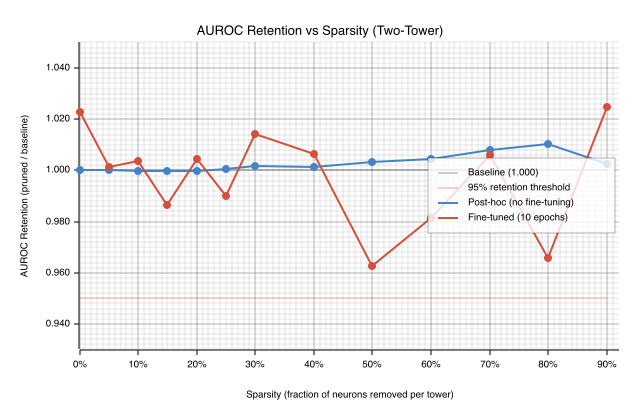
\includegraphics[width=\linewidth]{figures/fig4_3_pruning_curve.png}
\caption{Sparsity vs AUROC retention for post-hoc (blue) and fine-tuned
(red) evaluations. The solid black line marks the baseline (1.000); the
solid red line marks the 95\% retention threshold. Post-hoc retention
never falls below 0.9996.}
\end{figure}

\begin{figure}
\centering
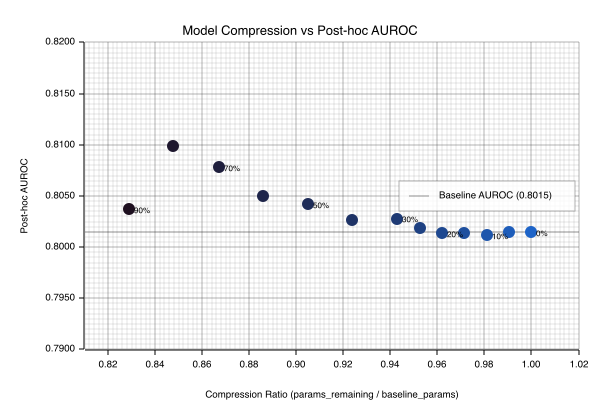
\includegraphics[width=\linewidth]{figures/fig4_4_compression_scatter.png}
\caption{Compression ratio vs post-hoc AUROC. Each point represents one
sparsity level; higher compression (lower ratio) corresponds to higher
sparsity. The horizontal reference line marks the baseline AUROC
(0.8015). Points above the line represent post-hoc improvements over the
unpruned model.}
\end{figure}

\textbf{Interpretation.} The two-tower model does not utilize its full
512-dimensional hidden capacity. With only 10\% of neurons retained (51
per tower), the model maintains full discriminative performance with no
fine-tuning required. Three factors likely contribute to this
redundancy:

First, the cosine similarity scoring objective constrains the useful
dimensionality of the representation. Since the regulatory score depends
only on the \emph{direction} of the TF and gene encodings (not their
magnitude), the effective number of degrees of freedom available to the
objective is at most the number of dimensions needed to arrange \(K\)
directional clusters, which for the GRN problem may be far smaller than
512.

Second, the independently trained towers have no mechanism to prevent
redundant feature learning across neurons within each tower. Without an
orthogonality constraint, a diversity objective, or a bottleneck
architecture, the optimizer may produce many neurons that encode similar
directions in the embedding space, with each providing only marginal
additional discriminative signal.

Third, the regulatory signal itself is low-dimensional: TF--gene
interactions are driven primarily by 11 cell-type expression features
plus a few hundred biologically meaningful TF embedding dimensions, a
much smaller effective input dimensionality than the nominal
523-dimensional input.

This finding connects causally to H1. If the two-tower cannot exploit
its full 512-unit hidden capacity due to the geometric constraints of
cosine similarity scoring, then the parameter-matching argument in its
favor is weaker than it appears: a nominally parameter-matched two-tower
may have substantially lower \emph{effective} capacity than a
cross-encoder. The cross-encoder, whose MLP scoring function can utilize
all weight dimensions through the nonlinear readout layer, is not
subject to the same constraint. Hypothesis 3 is supported.

\section{4.7 Discussion}\label{discussion}

The three hypotheses investigated in this chapter form a coherent
account of the relationship between architectural inductive bias and
representational efficiency in neural GRN inference. The cross-encoder's
advantage over the two-tower (H1) is robust to realistic class imbalance
where the two-tower fails (H2), and the pruning analysis explains
\emph{why} the two-tower is limited: its nominal parameter count does
not reflect its effective capacity (H3).

\textbf{Unified interpretation.} The factorized two-tower architecture
imposes a strong inductive bias that is both its strength and its
weakness. By separating TF and gene encoding, the two-tower enables
efficient inference at scale: given pre-computed TF and gene embeddings,
all \(M \times N\) TF--gene regulatory scores can be computed as a
matrix product in \(O(Md + Nd)\) time rather than the \(O(MNd)\)
required by per-pair cross-encoder inference. This scalability property
is genuine and relevant for genome-scale GRN inference over tens of
thousands of gene pairs. However, the cosine-similarity scoring
mechanism that enables this efficiency also prevents the model from
learning the joint features that drive regulatory specificity, leading
to the AUROC gap observed in H1 and the sensitivity to class imbalance
in H2.

The neuron pruning results (H3) reinforce this picture: the two-tower's
512-dimensional hidden space is far larger than necessary, suggesting
that the cosine similarity objective cannot leverage the
representational capacity that is nominally available. This provides a
mechanistic account of the H1 AUROC gap that goes beyond simply noting
that the cross-encoder has a more expressive scoring function. The
two-tower is not just less expressive in principle --- it actively fails
to use the capacity it has.

\textbf{Practical recommendations.} For practitioners choosing between
two-tower and cross-encoder architectures for GRN inference:

\begin{itemize}
\tightlist
\item
  If AUROC and discriminative performance are the primary criteria, and
  the evaluation dataset has a realistic negative sampling ratio, the
  cross-encoder is the clear choice.
\item
  If scalability is paramount --- for example, in genome-scale
  applications requiring \(10^6\)--\(10^8\) pair evaluations --- the
  two-tower may be preferred, but practitioners should be aware of the
  6--10 AUROC point performance cost relative to a cross-encoder of
  comparable size, and should consider using only the compressed
  (pruned) two-tower, which achieves the same performance at 83\% of the
  original parameter count.
\end{itemize}

\textbf{Limitations.} Several limitations constrain the generalizability
of these findings. This study uses a single biological dataset (human
brain single-nucleus RNA-seq); whether the cross-encoder advantage
persists across other tissues, organisms, or expression modalities is
not established. Training was performed on CPU hardware, which
constrains the scale of architectures that could be practically
evaluated; larger models with wider hidden layers or additional depth
might close the AUROC gap. The two-tower architecture tested here uses
cosine similarity with temperature scaling; alternative scoring
functions such as bilinear similarity or attention-based cross-tower
interaction might recover some of the expressiveness lost to the cosine
similarity bottleneck. The pruning experiment was conducted at a single
seed; multi-seed pruning was not evaluated, and the non-monotonic
fine-tuning behavior suggests that the 10-epoch fine-tune budget is
insufficient to fully characterize the relationship between sparsity and
performance. Finally, the pruning analysis characterizes only the fc1
output neurons; fc2 output neurons and the embedding tables were not
pruned, and their redundancy is unknown.

\textbf{Future directions.} Three extensions are directly motivated by
these results. First, an InfoNCE-trained two-tower, where the
contrastive objective explicitly attracts positive TF--gene pairs and
repels negatives within a batch, may be more robust to the marginal
distribution sensitivity observed in H2 while retaining the two-tower's
inference efficiency. Second, Deep Mutual Learning between two decoders
may address the redundancy problem (H3) by introducing a diversity
pressure through the agreement regularization term. Third, a
cross-attention two-tower --- where the gene encoder attends over the TF
encoding before producing a final representation --- would bridge the
two architectures, enabling per-pair interaction features while
maintaining the factorized structure required for efficient inference.

\section{4.8 Conclusion}\label{conclusion}

This chapter has presented a systematic experimental comparison of
two-tower and cross-encoder neural architectures for TF--gene regulatory
edge prediction from single-cell RNA-seq data. Under parameter-matched,
data-matched conditions, the cross-encoder achieves 9.4 higher AUROC
points than the two-tower under balanced training (0.9040 vs 0.8097), is
robust to 5:1 class imbalance where the two-tower degrades by 6.6 AUROC
points, and demonstrates substantially more stable training (2.6× lower
standard deviation at 5:1). A neuron pruning analysis further shows that
the two-tower's 512-dimensional hidden space is nearly entirely
redundant: post-hoc AUROC never falls below the 95\% retention threshold
at any tested sparsity level, and 51 neurons per tower (10\% of the
original 512) suffice to match baseline performance with no additional
training.

Together, these results indicate that the cross-encoder is the more
appropriate choice for GRN inference tasks where discriminative accuracy
is paramount, while the two-tower offers a scalable inference-efficient
alternative whose performance can be maintained at substantially reduced
model size through structured pruning. The mechanistic link between H1
and H3 --- that the two-tower's AUROC deficit reflects wasted capacity
due to cosine similarity's geometric constraints --- provides a
principled foundation for future work on architectures that combine the
efficiency of factorized encoding with the expressiveness of joint
interaction features.

\section{4.9 References}\label{references}

Aibar, S., González-Blas, C. B., Moerman, T., Imrichová, H., Hulselmans,
G., Rambow, F., \ldots{} \& Aerts, S. (2017). SCENIC: single-cell
regulatory network inference and clustering. \emph{Nature Methods},
14(11), 1083--1086.

Bromley, J., Guyon, I., LeCun, Y., Säckinger, E., \& Shah, R. (1993).
Signature verification using a ``Siamese'' time delay neural network.
\emph{Advances in Neural Information Processing Systems}, 6.

Frankle, J., \& Carlin, M. (2019). The lottery ticket hypothesis:
Finding sparse, trainable neural networks. \emph{International
Conference on Learning Representations (ICLR)}.

García-Alonso, L., Holland, C. H., Ibrahim, M. M., Turei, D., \&
Saez-Rodriguez, J. (2019). Benchmark and integration of resources for
the estimation of human transcription factor activities. \emph{Genome
Research}, 29(8), 1363--1375.

Han, S., Pool, J., Tran, J., \& Dally, W. (2015). Learning both weights
and connections for efficient neural networks. \emph{Advances in Neural
Information Processing Systems}, 28.

Han, H., Cho, J. W., Lee, S., Yun, A., Kim, H., Bae, D., \ldots{} \&
Lee, I. (2018). TRRUST v2: an expanded reference database of human and
mouse transcriptional regulatory interactions. \emph{Nucleic Acids
Research}, 46(D1), D380--D386.

Huang, P. S., He, X., Gao, J., Deng, L., Acero, A., \& Heck, L. (2013).
Learning deep structured semantic models for web search using
clickthrough data. \emph{Proceedings of the 22nd ACM International
Conference on Information \& Knowledge Management (CIKM)}, 2333--2338.

Huynh-Thu, V. A., Irrthum, A., Wehenkel, L., \& Geurts, P. (2010).
Inferring regulatory networks from expression data using tree-based
methods. \emph{PLOS ONE}, 5(9), e12776.

Kingma, D. P., \& Ba, J. (2015). Adam: A method for stochastic
optimization. \emph{International Conference on Learning Representations
(ICLR)}.

Nogueira, R., \& Cho, K. (2019). Passage re-ranking with BERT.
\emph{arXiv preprint arXiv:1901.04085}.

Humeau, S., Shuster, K., Lachaux, M.-A., \& Weston, J. (2020).
Poly-encoders: Architectures and pre-training strategies for fast and
accurate multi-sentence scoring. \emph{International Conference on
Learning Representations (ICLR)}.

Khattab, O., \& Zaharia, M. (2020). ColBERT: Efficient and effective
passage search via contextualized late interaction over BERT.
\emph{Proceedings of the 43rd International ACM SIGIR Conference on
Research and Development in Information Retrieval}, 39--48.

\protect\phantomsection\label{refs}
\begin{CSLReferences}{1}{1}
\bibitem[\citeproctext]{ref-aibar2017}
{Aibar, Sara, Carmen Bravo González-Blas, Thomas Moerman, et al.} 2017.
{``{SCENIC}: Single-Cell Regulatory Network Inference and Clustering.''}
\emph{Nature Methods} 14 (11): 1083--86.

\bibitem[\citeproctext]{ref-bromley1993}
Bromley, Jane, Isabelle Guyon, Yann LeCun, Eduard Säckinger, and Roopak
Shah. 1993. {``Signature Verification Using a {`{Siamese}'} Time Delay
Neural Network.''} \emph{Advances in Neural Information Processing
Systems} 6.

\bibitem[\citeproctext]{ref-chen2016}
Chen, Tianqi, and Carlos Guestrin. 2016. {``{XGBoost}: {A} Scalable Tree
Boosting System.''} \emph{Proceedings of the 22nd ACM SIGKDD
International Conference on Knowledge Discovery and Data Mining},
785--94.

\bibitem[\citeproctext]{ref-frankle2019}
Frankle, Jonathan, and Michael Carlin. 2019. {``The Lottery Ticket
Hypothesis: {Finding} Sparse, Trainable Neural Networks.''}
\emph{International Conference on Learning Representations (ICLR)}.

\bibitem[\citeproctext]{ref-garcia2019}
García-Alonso, Luz, Christian H. Holland, Mahmoud M. Ibrahim, Dénes
Turei, and Julio Saez-Rodriguez. 2019. {``Benchmark and Integration of
Resources for the Estimation of Human Transcription Factor
Activities.''} \emph{Genome Research} 29 (8): 1363--75.

\bibitem[\citeproctext]{ref-han2018}
{Han, Heonjong, Jae-Won Cho, Sangyeon Lee, et al.} 2018. {``{TRRUST} V2:
An Expanded Reference Database of Human and Mouse Transcriptional
Regulatory Interactions.''} \emph{Nucleic Acids Research} 46 (D1):
D380--86.

\bibitem[\citeproctext]{ref-han2015}
Han, Song, Jeff Pool, John Tran, and William Dally. 2015. {``Learning
Both Weights and Connections for Efficient Neural Networks.''}
\emph{Advances in Neural Information Processing Systems} 28.

\bibitem[\citeproctext]{ref-huang2013}
Huang, Po-Sen, Xiaodong He, Jianfeng Gao, Li Deng, Alex Acero, and Larry
Heck. 2013. {``Learning Deep Structured Semantic Models for Web Search
Using Clickthrough Data.''} \emph{Proceedings of the 22nd ACM
International Conference on Information \& Knowledge Management (CIKM)},
2333--38.

\bibitem[\citeproctext]{ref-humeau2020}
Humeau, Samuel, Kurt Shuster, Marie-Anne Lachaux, and Jason Weston.
2020. {``Poly-Encoders: Architectures and Pre-Training Strategies for
Fast and Accurate Multi-Sentence Scoring.''} \emph{International
Conference on Learning Representations (ICLR)}.

\bibitem[\citeproctext]{ref-huynh2010}
Huynh-Thu, Vân Anh, Alexandre Irrthum, Louis Wehenkel, and Pierre
Geurts. 2010. {``Inferring Regulatory Networks from Expression Data
Using Tree-Based Methods.''} \emph{PLOS ONE} 5 (9): e12776.

\bibitem[\citeproctext]{ref-khattab2020}
Khattab, Omar, and Matei Zaharia. 2020. {``{ColBERT}: Efficient and
Effective Passage Search via Contextualized Late Interaction over
{BERT}.''} \emph{Proceedings of the 43rd International ACM SIGIR
Conference on Research and Development in Information Retrieval},
39--48.

\bibitem[\citeproctext]{ref-kingma2014}
Kingma, Diederik P., and Jimmy Ba. 2015. {``Adam: {A} Method for
Stochastic Optimization.''} \emph{International Conference on Learning
Representations (ICLR)}.

\bibitem[\citeproctext]{ref-nogueira2019}
Nogueira, Rodrigo, and Kyunghyun Cho. 2019. {``Passage Re-Ranking with
{BERT}.''} \emph{arXiv Preprint arXiv:1901.04085}.

\end{CSLReferences}

\end{document}
